\documentclass{beamer}

\input{../preambulo/inputenc.tex}
\input{../preambulo/fuente.tex}
\input{../preambulo/spanish.tex}
\input{../preambulo/tikz.tex}
\input{../preambulo/matematica.tex}
\input{../preambulo/colors.tex}
\input{../preambulo/flotantes.tex}
\input{../preambulo/beamer_zub.tex}
\input{../preambulo/paquetes.tex}
\usepackage{ccicons}
% \ccPublicDomain

\newcommand{\etal}{{\it et al.}}
\newcommand{\ie}{{\it i. e.}}
\newcommand{\zlink}[1]{\href{#1}{\color{celeste}\faExternalLink*}}


\graphicspath{{../img/}{img/}}
\framebg{bg/pizarron3.png} 
\hypersetup{colorlinks=true, urlcolor=azul!40!white}

\begin{document}

\newcommand\CC{}

\begin{zframe}{}% yscale=0.9, % with frametitle
\path(cp) ++(3,0) node(I)[]{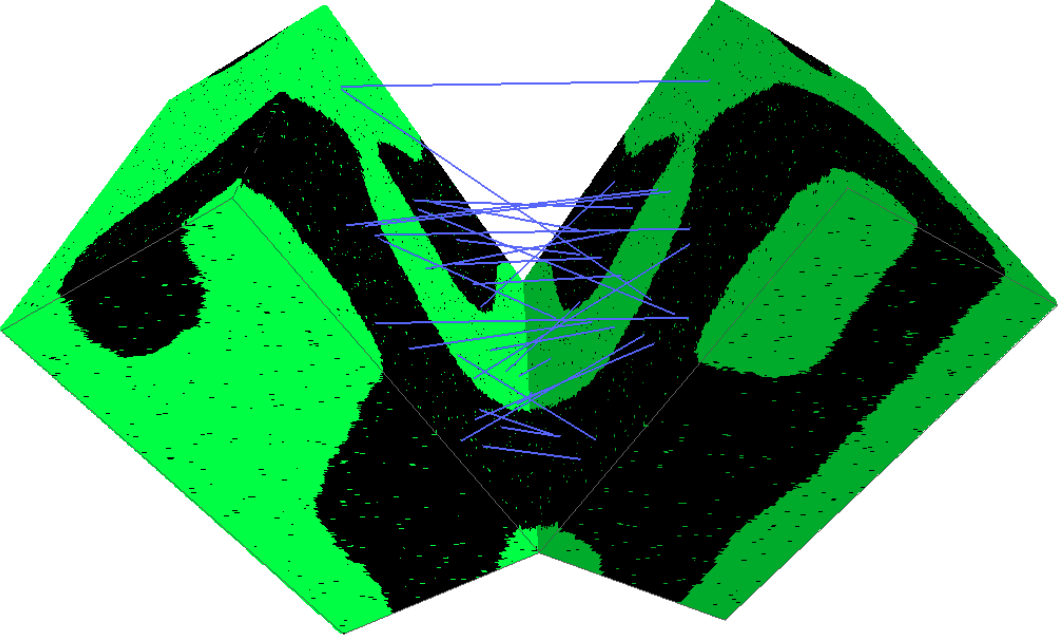
\includegraphics[angle=90,width=4.5cm]{img/ising3Dsplit.png}};
\path(c2|-I.north) ++(0,-.5) node(A)[anchor=north,align=left]{
  \color{verde} \large\textbf{Métodos Computacionales}\\[3mm]  
  \color{celeste} \textbf{Cadenas de Markov}\\[2mm]  
  \color{lila} \textit{Octubre 20, 2025}
};
\normalsize
\path(A.west|-I.south) ++(0,.5) node(B)[anchor=south west,align=left]{
  S. Alexis Paz\\[5mm]

\includegraphics[width=3cm]{logos/DQTC_orange.png}};

\path(I.south east) ++(0,0) node[anchor=north east,inner sep=0]{
  \tiny Leist \textit{et al.}, \href{https://doi.org/10.1016/j.jocs.2010.04.001}{J.Comp.Sc. 1(2010)33}};
 
% Referencia de la Foto del Ising 3D
% SP Singh, A Kumari Singh, Formation of liquid structures and investigation of
% its interfacial properties using lattice based liquid-gas model, Proceedings of
% International Conference on Nanoscience and Nanotechnology, 29th Nov.-01st Dec.
% 2019, VIT, Vellore, Tamil Nadu, India
 
\end{zframe}

\renewcommand\CC{
  \path(se) node[anchor=south east]{\tiny\color{gray} MC2025 - S.A.Paz};}
               
\begin{zframe}{}
\node[zf/title=center]{Monte Carlo en Química Computacional};

\node[zf/text=middle,amarillo]{
 $\ds\ab<\dfrac{f(X)}{q(X)}>=\int_{\Omega}f(x)\odif{x}\approx\avg{\ab(\dfrac{f(X)}{q(X)})}$ };

\draw[celeste,ultra thick,<-|](text.west) -- ++(-1,0) -- ++(0,1) coordinate(x); 

\node[zf/text=return]{Pero... ¿Que que integral queremos {\color{celeste}computar}?};

\path(text.east) -- ++(1.4,0) coordinate(xx);
\draw[celeste,ultra thick,<-|](text.east) -- (xx) -- (xx|-x); 

\node[zf/text=middle,amarillo]{
 $\ds\ab<A>=\int_{\Omega}a(\vb{x})\rho(\vb{x})\odif{\vb{x}}\approx\avg{\ab(\dfrac{a(\vb{X})\rho(\vb{X})}{q(\vb{X})})}$ };

\path(last.east) ++(.2,0) node(A)[celeste,anchor=west,align=left]{$\leftarrow$ Mecánica\\  \hspace{5mm} Estadística};

\node[zf/text=return]{Usualmente elegimos $q(\vb{x})=\rho(\vb{x})$};

\path(last.east) ++(.2,0) node(A)[celeste,anchor=west,align=left]{$\leftarrow$ Muestreo de Importancia};

\node[zf/text=middle,amarillo]{
 $\ds\ab<A>\approx\avg{a(\vb{X})}\qquad \vb{X}\sim\rho(\vb{x})$};

\path(last.east) ++(.2,-.2) node(A)[celeste,anchor=west,align=left]{$\leftarrow$ Ensamble\\ \hspace{5mm}termodinámico};

\node[zf/text=middle,naranja,shift={(0,-1)}]{\Large Tenemos que generar $\vb{X}\sim\rho(\vb{x})$\ldots``muestrear $\rho(\vb{x})$''};

\end{zframe}
                 
\begin{zframe}{}

\node[zf/title=center]{Generar $\vb{X}\sim\rho(\vb{x})$};

\node[zf/text=return,shift={(0,-.8)}]{Pero... $\vb{X}\in\mathcal{R}^{3N}$};

\node[zf/text=next,shift={(0,-.6)}]{TTVA no se puede};

\node[zf/text=next,shift={(0,-.6)}]{¡Método del rechazo!};

\node[zf/text=next,shift={(0,-.6)}]{Pero $\mathcal{R}^{3N}$ es enorme y solo algunas regiones son interesantes};

\node[zf/text=middle,shift={(0,-.6)},verde]{¿Cómo genero $\vb{X}$ que no se rechacen siempre?};




\path(vu) ++(1,-1) coordinate(A);

\begin{scope}[rotate=0,thick,shift={(A)}]

  % current minima
  \pgfmathsetseed{123456}
  \pgfmathsetmacro{\rad}{2.0}
  \pgfmathsetmacro{\xy}{0.9*\rad}
  \path(0,0) coordinate (A1);
  \path(A1) node[rotate=30,penciline={jag ratio=0},draw=celeste,ellipse,minimum height=\rad*10,minimum width=\xy*10]{};  
  \path(A1) node[rotate=30,penciline={jag ratio=0},draw=celeste,ellipse,minimum height=\rad*20,minimum width=\xy*20]{};  
  \path(A1) node[rotate=30,penciline={jag ratio=0},draw=celeste,ellipse,minimum height=\rad*30,minimum width=\xy*30]{};  
  \path(A1) node[rotate=30,penciline={jag ratio=0},draw=celeste,ellipse,minimum height=\rad*40,minimum width=\xy*40]{};  

  % neighboor minima 1
  \pgfmathsetseed{321346}
  \pgfmathsetmacro{\rad}{1.6}
  \pgfmathsetmacro{\xy}{1.1*\rad}
  \path(3,0.5) coordinate (A2);
  \path(A2) node[rotate=30,penciline={jag ratio=0},draw=celeste,ellipse,minimum height=\rad*10,minimum width=\xy*10]{};  
  \path(A2) node[rotate=30,penciline={jag ratio=0},draw=celeste,ellipse,minimum height=\rad*20,minimum width=\xy*20]{};  
  \path(A2) node[rotate=30,penciline={jag ratio=0},draw=celeste,ellipse,minimum height=\rad*30,minimum width=\xy*30]{};  
       
  % neighboor minima 2
  \pgfmathsetseed{879821}
  \pgfmathsetmacro{\rad}{1.2}
  \pgfmathsetmacro{\xy}{1.1*\rad}
  \path(-1,-2.5) coordinate (A3);
  \path(A3) node[rotate=30,penciline={jag ratio=0},draw=celeste,ellipse,minimum height=\rad*10,minimum width=\xy*10]{};  
  \path(A3) node[rotate=30,penciline={jag ratio=0},draw=celeste,ellipse,minimum height=\rad*20,minimum width=\xy*20]{};  
  \path(A3) node[rotate=30,penciline={jag ratio=0},draw=celeste,ellipse,minimum height=\rad*30,minimum width=\xy*30]{};  

  % Transition line 1
  \pgfmathsetseed{834297}
  \path(A1) +($(A1)!0.6!(A3)$) +([turn]90:1) coordinate(aux1);
  \path(A1) +($(A1)!0.6!(A3)$) +([turn]-90:1) coordinate(aux2);
  \draw[penciline={jag ratio=0},draw=celeste,] (aux1) -- (aux2);

  % Transition line 2
  \pgfmathsetseed{134127}
  \path(A1) +($(A1)!0.55!(A2)$) +([turn]90:1) coordinate(aux1);
  \path(A1) +($(A1)!0.55!(A2)$) +([turn]-90:1) coordinate(aux2);
  \draw[penciline={jag ratio=0},draw=celeste,] (aux1) -- (aux2);

  % Trajectory on first minima
  \pgfmathsetmacro{\rad}{0.3}
  \pgfmathsetseed{169221}
  \foreach \c in {0,...,30}{
    \path(A1) ++({\rad*(rand+rand+rand+rand+rand)},{\rad*(rand+rand+rand+rand+rand)}) coordinate (sum-\c);
  }

  \path(A1) +($(A1)!0.2!(A2)$) coordinate (sum-31);
  \path(A1) +($(A1)!0.4!(A2)$) +([turn]-30:0.5) coordinate (sum-32);
  \path(A1) +($(A1)!0.6!(A2)$) +([turn]30:0.5) coordinate (sum-33);
  \path(A2) coordinate (sum-34);
     
  \pgfmathsetseed{932121}
  \pgfmathsetmacro{\rad}{0.2}
  \foreach \c in {35,...,50}{
    \path(A2) ++({\rad*(rand+rand+rand+rand+rand)},{\rad*(rand+rand+rand+rand+rand)}) coordinate (sum-\c);
  }
       
  \def\pts{}
  \foreach \x in {0,...,50} { \xdef\pts{\pts (sum-\x)}; }

  \draw[naranja] plot[smooth] coordinates {\pts};

\end{scope}
      

\end{zframe}
                 
\begin{zframe}{}
                          
\path<1-3>(cp) ++(0,0) node(A){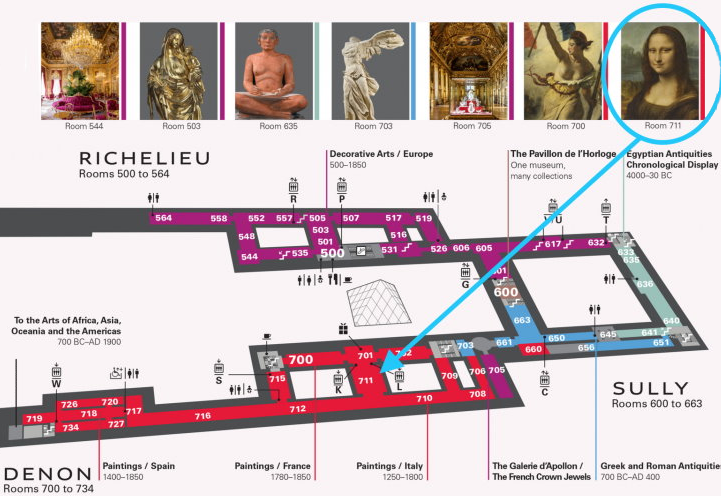
\includegraphics[width=12cm]{louvre.png}};

\only<2->{
% Richelieu
\fill[amarillo](3.1,5.3)                  circle(.1) coordinate(R1);
\fill[amarillo,ultra thick](R1) ++(0:1)   circle(.1) coordinate(R2);
\fill[amarillo,ultra thick](R1) ++(0:1.5) circle(.1) coordinate(R3);
\fill[amarillo,ultra thick](R1) ++(0:2.0) circle(.1) coordinate(R4);
\fill[amarillo,ultra thick](R1) ++(0:2.5) circle(.1) coordinate(R5);
\fill[amarillo,ultra thick](R1) ++(0:3.1) circle(.1) coordinate(R6);
\fill[amarillo,ultra thick](R1) ++(0:3.8) circle(.1) coordinate(R7);
\fill[amarillo,ultra thick](R1) ++(0:4.3) circle(.1) coordinate(R8);
                                        
% Richelieu 2
\fill[amarillo,ultra thick](R3) ++(0,-.6)  circle(.1) coordinate(R9);
\fill[amarillo,ultra thick](R9) ++(2:0.7) circle(.1) coordinate(R10);
\fill[amarillo,ultra thick](R9) ++(2:1.3) circle(.1) coordinate(R11);
\fill[amarillo,ultra thick](R9) ++(2:2.3) circle(.1) coordinate(R12);
\fill[amarillo,ultra thick](R9) ++(2:3.1) circle(.1) coordinate(R13);
\fill[amarillo,ultra thick](R9) ++(2:3.5) circle(.1) coordinate(R14);
\fill[amarillo,ultra thick](R9) ++(2:3.9) circle(.1) coordinate(R15);
\fill[amarillo,ultra thick](R9) ++(2:4.9) circle(.1) coordinate(R16);
\fill[amarillo,ultra thick](R9) ++(2:5.9) circle(.1) coordinate(R17);
                                        
% Denon
\fill[amarillo,ultra thick](1.6,1.8)      circle(.1) coordinate(D1);
\fill[amarillo,ultra thick](D1) ++(5:.7)  circle(.1) coordinate(D2);
\fill[amarillo,ultra thick](D1) ++(5:2.2) circle(.1) coordinate(D3);
\fill[amarillo,ultra thick](D1) ++(5:3.8) circle(.1) coordinate(D4);
\fill[amarillo,ultra thick](D1) ++(5:5.9) circle(.1) coordinate(D5);
\fill[amarillo,ultra thick](D1) ++(5:6.8) circle(.1) coordinate(D6);
 
% Denon2
\fill[amarillo,ultra thick](D4) ++(0,.8)  circle(.1) coordinate(D7);
\fill[amarillo,ultra thick](D7) ++(5:1.1) circle(.1) coordinate(D8);
\fill[amarillo,ultra thick](D7) ++(5:1.7) circle(.1) coordinate(D9);
\fill[amarillo,ultra thick](D7) ++(5:2.8) circle(.1) coordinate(D10);
\fill[amarillo,ultra thick](D7) ++(5:3.4) circle(.1) coordinate(D11);
\fill[amarillo,ultra thick](D7) ++(5:4.3) circle(.1) coordinate(D12);
\fill[amarillo,ultra thick](D7) ++(5:5.1) circle(.1) coordinate(D13);
                                       
% Mona
\fill[amarillo,ultra thick](D8) ++(.1,-.5) circle(.1) coordinate(D14);
}

\only<3->{
% \foreach \x in {1,2,...,7}{
%   \pgfmathsetmacro\xx{\x+1)}
%   \pgfmathsetmacro\xxx{\x+2)}
%   \pgfmathsetmacro\xxxx{\x+9)}
%   \pgfmathsetmacro\xxxxx{\x+10)}
   \pgfmathsetmacro\tr{1}%random()}
%   \foreach \y in {\x,\xx,\xxx,\xxxx,\xxxxx}{
%     % \pgfmathsetmacro\y{\x+1)}
%     \draw[thick,amarillo,opacity=\tr] (R\x) -- (R\y);
%   }
% }
% \foreach \x in {1,2,...,7}{
%     \pgfmathsetmacro\y{\x+1)}
%     \draw[thick,amarillo,opacity=\tr] (R\x) -- (R\y);
% }
% \foreach \x in {9,10,...,16}{
%     \pgfmathsetmacro\y{\x+1)}
%     \draw[thick,amarillo,opacity=\tr] (R\x) -- (R\y);
% }
\draw[thick,verde,opacity=\tr] (R1) -- (R8);
\draw[thick,verde,opacity=\tr] (R9) -- (R17);
\draw[thick,verde,opacity=\tr] (D1) -- (D6);
\draw[thick,verde,opacity=\tr] (D7) -- (D13);

\draw[thick,verde,opacity=\tr] (D4) -- (D8);
                   
\foreach \x in {14,...,17}{
  \foreach \y in {9,...,13}{
    \draw[thick,verde,opacity=\tr] (R\x) -- (D\y);
  }
}                  
\foreach \x in {4,...,9}{
  \foreach \y in {4,14}{
    \draw[thick,verde,opacity=\tr] (R\x) -- (D\y);
  }
}
\foreach \x in {1,...,2}{
  \foreach \y in {1,2,3,4,14}{
    \draw[thick,verde,opacity=\tr] (R\x) -- (D\y);
  }
}
\foreach \x in {4,...,6}{
  \draw[thick,verde,opacity=\tr] (D\x) -- (D14);
}
}

\path<7>(vu) ++(0,.5) node[text width=11cm, align=center]
{En un instante $t$ la probabilidad de estar en $x_i$ es\\[2mm]
  ${\rho_i(t)=P\ab[X=x_i(t)]}$\\[2mm]
};
          
\path<6>(vu) ++(0,.5) node(T)[texto,anchor=north]{
  $X_1\rightarrow X_2\rightarrow X_3\rightarrow X_4\rightarrow X_5\rightarrow \cdots$\\[2mm]
\color{naranja}\textit{¡Caminar es una forma de generar estados aleatorios!}
};        

\path<4->(R1) node[amarillo,above]{$x_1$};
\path<4->(D1) node[amarillo,left]{$x_2$};
\path<4->(R2) node[amarillo,above]{$x_3$};
\path<4->(D2) node[amarillo,below]{$x_4$};
\path<4->(D3) node[amarillo,below]{$x_5$};
\path<4->(R8) node[amarillo,above]{$x_n$};

\path<5>(vu) ++(0,.5) node[text width=11cm, align=center]
{La trayectoria $x(t)$ de un caminante forma una cadena de estados\\[2mm] 
  $x_1(t_0)\rightarrow x_2(t_1)\rightarrow x_1(t_2)\rightarrow x_3(t_3)\rightarrow x_3(t_4)\rightarrow \cdots$\\[2mm] 
   forma una cadena de estados
};
 
% \path<5->(c2) ++(0,.5) node{$P_t(\rho_1,\rho_2,\cdots,\rho_n)$};
\path<8>(vu) ++(0,.5) node[text width=11cm, align=center]{
  Estando en $x_i$ a tiempo $t_0$, la probabilidad de pasar a $x_j$ en $t_1$ es\\[2mm] 
  ${t_{i,j}^{(1)}=P[X=x_j(t_1)|x_i(t_0),x_k(t_{-1}),\cdots,x_m(t_{-n})]}$\\[2mm]
};

\path<9>(vu) ++(0,.5) node[text width=11cm, align=center]{
  En un proceso de Markov, la probabilidad de transición no depende de estados pasados\\[2mm]
  ${t_{i,j}^{(1)}=P[X=x_j|x_i]}$\\[2mm]
   \textit{Como todo proceso determinista}
};
 
% \path<6->(R1) -- (D1) node[pos=.5,left,celeste]{$\rho_{1,2}^{(1)}$};
% \path<6->(D2) -- (D3) node[pos=.5,below,amarillo]{$\rho_{4,5}^{(1)}$};




% \path<7->(vu) ++(0,.5) node{¿Cuál es la probabilidad de 
%   esta en el estado 1 pase al estado x?};

% \path<6->(c1) ++(0,.5) node{$\pxmat[showleft=2,showtop=2]{\rho}{n}{n}$};
                          
                          
\end{zframe}
          
\begin{zframe}{}

\node[zf/title=center]{\LARGE Ecuación Maestra};

\node[zf/text=return]{
  Puedo armar un vector con la probabilidad en cada estado\\[2mm]
  y una matriz con las transiciones\ldots};

\node[zf/text=return]{
  $\rho(t)=\begin{pmatrix}
  \rho_1(t)\\
  \rho_1(t)\\
  \vdots\\
  \rho_n(t)\end{pmatrix}$
};

\path(last-|te) node(T)[zf/text,anchor=east]{
  $\vb{T}=\pxmat[showleft=2,showtop=2]{t}{n}{n}$
};
 
\node(T)[zf/text=return,align=center]{
  La evolución de las probabilidades siguen la ecuación maestra:\\[2mm]
  $\ds\odv{\rho(t)}{t}=\vb{T}\rho(t)$\\[2mm]
  $\vb{T}$ es independiente del tiempo en un proceso de Markov.
};
   
\end{zframe}
           
\begin{zframe}{
  titulo/.style={verde, align=center},
}
 \large 

\path(cp|-t) ++(0,0) node(T)[titulo]{
\LARGE En equilibrio\ldots};

\path(t|-T.south) ++(0,-.5) node(T)[texto,text width=11cm]{
  $${\ds\odv{\rho(t)}{t}=\vb{T}\rho(t)=0\quad\Rightarrow\quad\sum_kt_{ik}\rho_i=0}$$
  El flujo de entrada y salida deben ser iguales
};

\path(t|-T.south) ++(0,-.5) node(T)[texto,text width=11cm]{
  Esto también se cumple con un {\color{verde}balance detallado}:
  \color{naranja}$${\ds t_{ji}\rho_i=t_{ij}\rho_j}$$
};
  
\end{zframe}
            
\begin{zframe}{
  titulo/.style={verde, align=center},
}
 \large 

\path(cp|-t) ++(0,.3) node(T)[titulo]{
\LARGE Metropolis–Hastings};

\path(cp|-T.south) ++(0,-.2) node(T)[texto,anchor=north]{
  Caminar \ldots$X_1(t_0)\rightarrow X_2(t_1)\rightarrow X_1(t_2)\rightarrow X_3(t_3)\rightarrow \cdots$\\[2mm]
\color{naranja}\textit{ para \textbf{muestrear} estados de equilibrio de un proceso Markoviano.}
};
 
\path(t|-T.south) ++(-.4,-.5) node(T)[texto,align=left]{
  1. Elijo un estado inicial $X_i$.\\[2mm]
  2. Perturbo $X_i$ para generar otro estado posible $X_j$.\\[2mm]
  3. Acepto ($X_i\rightarrow X_j$) con una cierta probabilidad, cumpliendo\\[2mm]
  \ \  con el balance detallado de la distribución de interés.\\[2mm]
  4.  Repito desde 2.\\[2mm] 
  5. \textit{La cadena resultante converge a esta distribucíon,}\\[2mm]
  \ \ \color{naranja}independientemente del estado $X_i$ inicial.};
 
\path(hr) ++(0,1.5) node(A)[celeste,align=center] {( $\rho$, $\vb{T}$, \cancel{pasado}, \cancel{$\vb{T}(t)$} )};

\path(c4) ++(1.3,.2) node(A)[rotate=-14,ellipse,celeste,ultra thick,inner sep=1,draw,align=center]
{¿Correlación? \\ no importa};

\end{zframe}

              
\begin{zframe}{
  titulo/.style={verde, align=center},
}
 \large 

\path(cp|-t) ++(0,.3) node(T)[titulo]{
\LARGE Metropolis–Hastings};

\path(T.south) ++(0,-.2) node(T)[texto,anchor=north,text width=11cm]{
 ¿Cual es la probabildad de transición?
  $${\ds t_{ji}=M(X_j|X_i)A(X_j|X_i)}$$\\
  pero por balance detallado ${\ds t_{ji}\rho_i=t_{ij}\rho_j}$
  $${\ds M(X_j|X_i)A(X_j|X_i)\rho_i=M(X_i|X_j)A(X_i|X_j)\rho_j}$$
  Eligiendo ${\ds M(X_j|X_i)=M(X_i|X_j)}$
  $${\ds A(X_j|X_i)\rho_i=A(X_i|X_j)\rho_j}$$
  Lo cual es siempre cierto si elijo
 \color{orange}$$\ds A(X_j|X_i)=\min\ab[1,\frac{\rho_j}{\rho_i}]$$
};

\end{zframe}
                              
\begin{zframe}{}

\node[zf/title=left]{Modelo de Ising};
\path<2->(last.east) ++(.3,0) node(A)[celeste,anchor=west]{(1D, Periódico, J constante)};

\node<1>[zf/text=next]{
  $\ds H = -\sum_{\langle i,j\rangle} J_{ij} s_i s_j -B \sum_{i}^N s_i \qquad s_i=\pm1$ };

\node<2->[zf/text=next]{
  $\ds H = -J \sum_{i=1}^{N} s_i s_{i+1}  -B \sum_{i=1}^N s_i \qquad s_i=\pm1, \quad s_{N+1}= s_1$ };
           
\node<3->[zf/text=next]{
  1. Elijo un estado inicial $\vb{s}_\alpha$. \color{celeste}$\leftarrow$ vector\only<8->{$\quad\vb{s}_i=\vb{X};\quad \vb{X}\sim\tilde\rho(X)$}
  \only<4-7>{\\[2mm]
           ¿$\vb{s}_\alpha=\vb{1}$?}\only<5-7>{\hspace{5mm}{\color{amarillo}$\sim$\ldots depende de J y B} \\[2mm]
           ¿$\vb{s}_\alpha=\vb{X};\qquad \vb{X}\sim\text{uniforme}$?}\only<6-7>{\hspace{5mm}\color{amarillo}$\sim$\ldots depende de J y B \\[2mm]
           ¿$\vb{s}_\alpha=\vb{X};\qquad \vb{X}\sim\rho(X)$?}\only<7>{\hspace{5mm}\color{rojo}\XSolidBrush\ldots no sabemos muestrear $\rho$ \\[2mm]
           ¿$\vb{s}_\alpha=\vb{X};\qquad \vb{X}\sim\tilde\rho(X)$?\hspace{5mm}{\color{verde}\Checkmark\ldots lo mas cercano posible}}
  };
       
\node<8->[zf/text=next]{
  2. Perturbo $\vb{s}_\alpha$ para generar $\vb{s}_\beta$.\color{celeste}\only<13->{\hspace{5mm}$s_i=-s_i; \quad i\sim\text{uniforme}$}
  \only<9-12>{\\[2mm]
           ¿$s_3=1$?}\only<10-12>{\hspace{5mm}\color{rojo}\XSolidBrush\ldots No es reversible   \\[2mm]
           ¿$s_3=-s_3$?}\only<11-12>{\hspace{5mm}\color{rojo}\XSolidBrush\ldots Arbitrario \\[2mm]
           ¿$s_i=-s_i; \quad i\sim\text{uniforme}$?}\only<12>{\hspace{5mm}{\color{verde}\Checkmark}\\[2mm]
           ¿$s_j=s_i; \quad j,i\sim\text{uniforme}$?\hspace{5mm}\color{amarillo}$\sim$ No es ``ergódico''} };

\node<13->[zf/text=next]{
  3. Acepto ($\vb{s}_\alpha\rightarrow \vb{s}_\beta$) con probabilidad $\min\ab[1,\frac{\rho(\vb{s}_\beta)}{\rho(\vb{s}_\alpha)}]$\\[2mm]
  \color{verde}$\rho\leftarrow$ ensamble (e.g. NVT)\color{celeste}\hspace{7mm} ¿$V$? pensar en $J=J(\text{distancia})=$cte};

\node<14->[zf/text=next]{
  4.  $\vb{s}_\alpha\Leftarrow \vb{s}_\beta$ y repito desde 2.\\[2mm] 
  5. \textit{La cadena converge a esta distribucíon, }\textit{\color{celeste}  ¿tiempo de convergencia?}\\[2mm]
  \ \ \color{naranja}independientemente del estado inicial. \textit{\color{celeste} ¿tiempo de correlación?}};
         
% \node[zf/text=next]{
% ¿Que ensamble quiero simular?\\};
%
% \node[zf/text=next]{
% ¿Que ensamble quiero simular?\\};
%

\end{zframe}
      
\begin{zframe}{}

\path(vu) ++(0,.5) node(I)[recorte]{\includegraphics[width=9cm]{review.png}};
\path(vl) ++(0,-.5) node(I)[recorte]{\includegraphics[width=9cm]{pame.png}};
\path(I.west) ++(-0.6,.1) node[naranja,rotate=90]{\sffamily EJEMPLO LOCAL};

\end{zframe}
                              
             
     
\end{document}
